\section{Evaluation}

\begin{figure*}
\centering
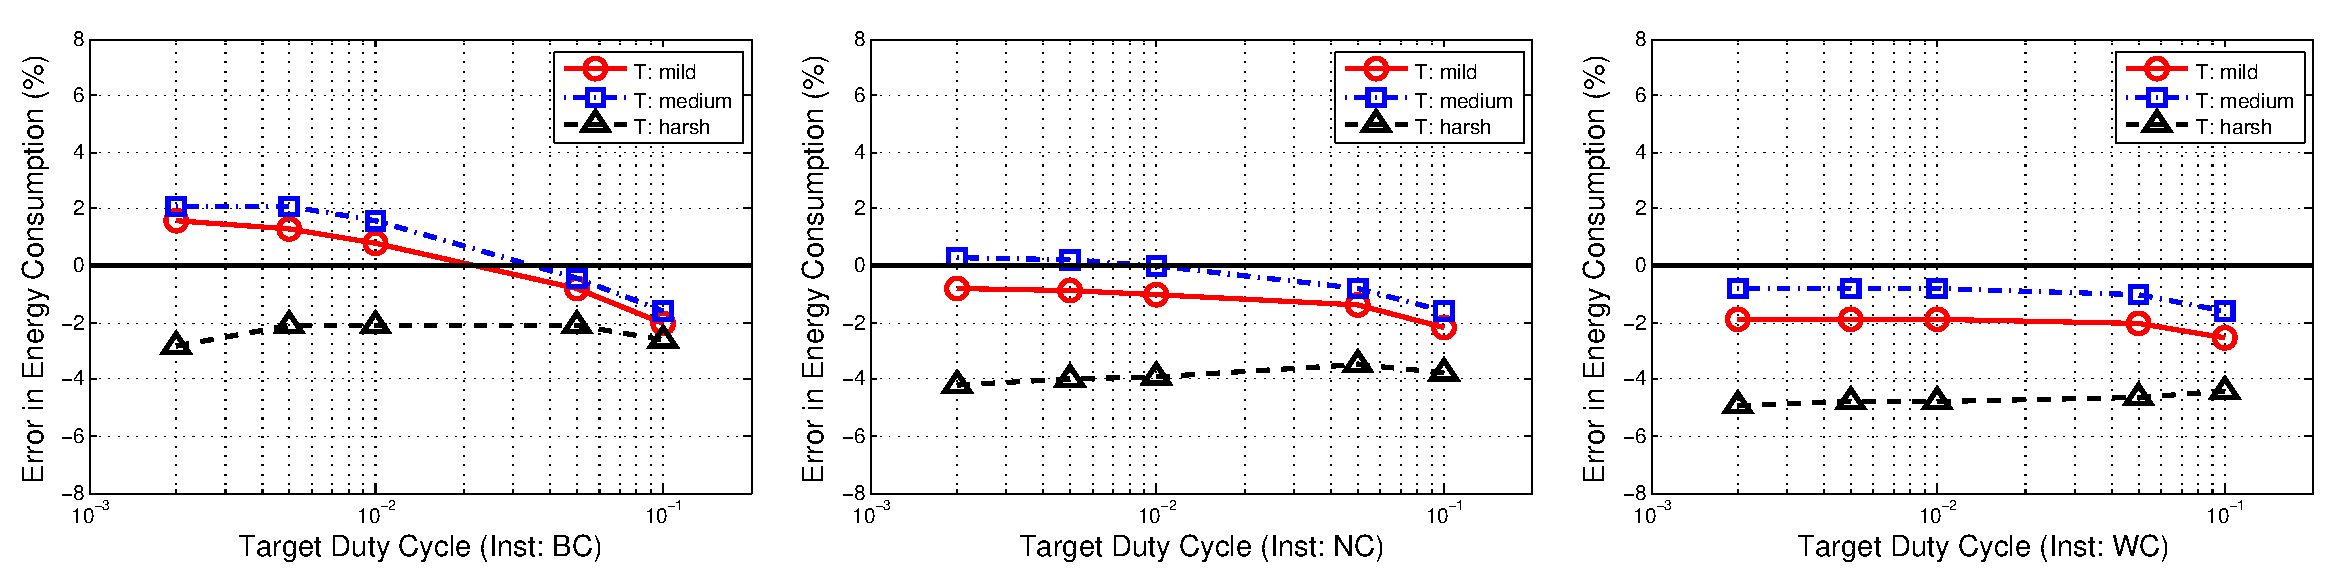
\includegraphics[width=1\textwidth]{figures/app1_nonoise.eps}
\caption{\label{fig:app1}App 1 results, no noise}
\end{figure*}

\begin{figure*}
\centering
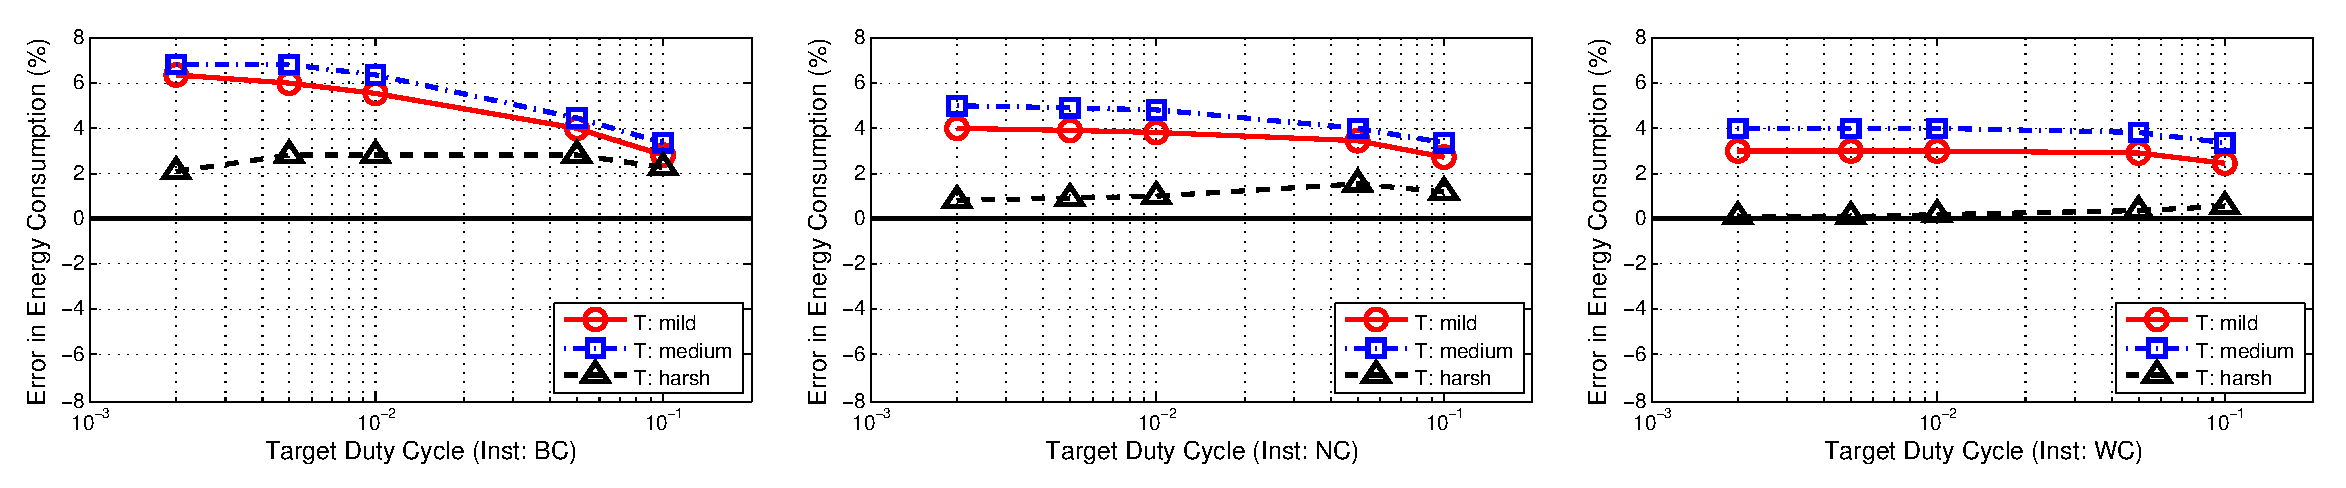
\includegraphics[width=1\textwidth]{figures/app1_guardband.eps}
\caption{\label{fig:app1}App 1 results, no noise}
\end{figure*}

\begin{figure}
\centering
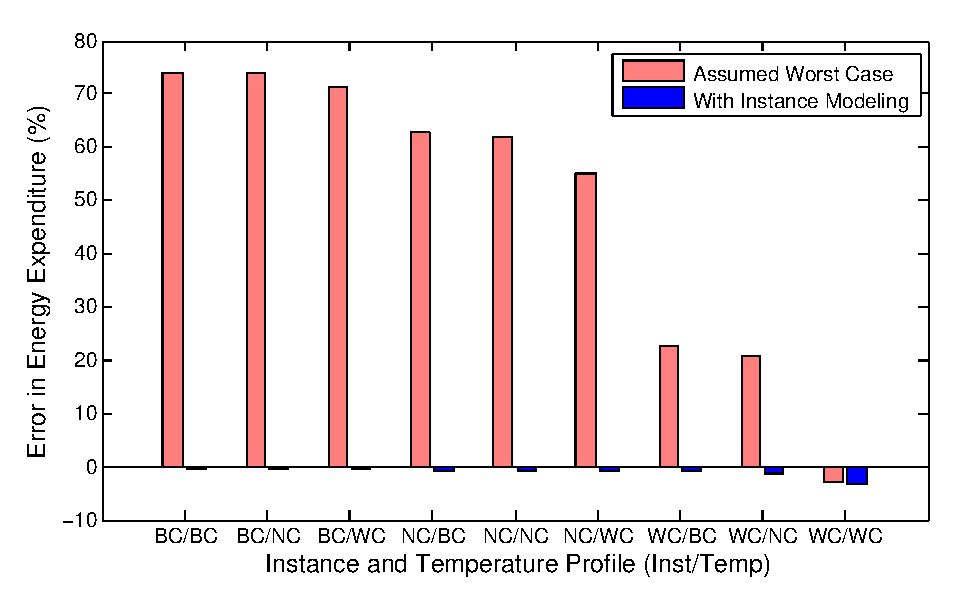
\includegraphics[width=1\columnwidth]{figures/app1_energycomp.eps}
\caption{\label{fig:app1}App 1 energy comparison}
\end{figure}

\begin{figure}
\centering
\includegraphics[width=1\columnwidth]{figures/app1_dutycycles.eps}
\caption{\label{fig:app1}App 1 dutycycle comparison}
\end{figure}

\begin{figure}
\centering
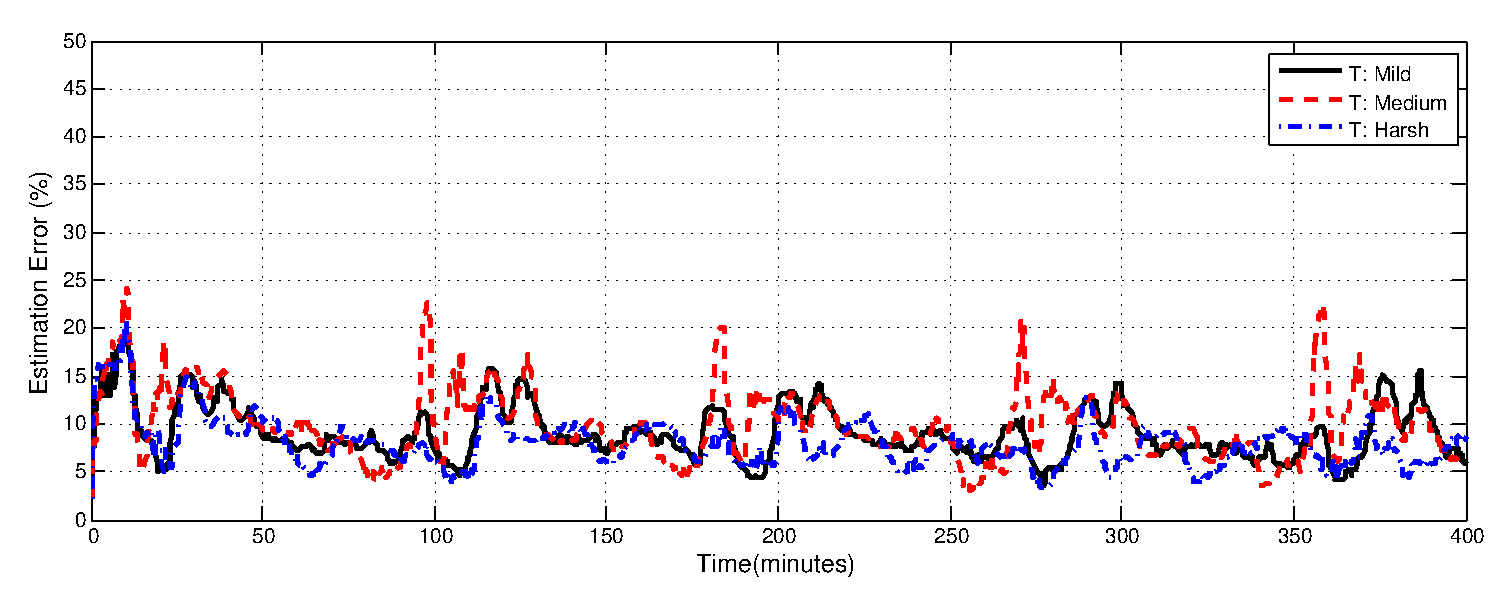
\includegraphics[width=1\columnwidth]{figures/localization_var.eps}
\caption{\label{fig:app1}App 1 dutycycle comparison}
\end{figure}



describe here the method of evaluation, introduce QEMU and VarEMU as tools for evaluation. Cite accuracy for varemu etc. 

\subsection{Multi-Sensor Applications}
Application 1: we have multiple sensors with various knobs fighting for resources with various utilities.

\subsection{Multi-Agent Applications}
Application 2: we have multiple agents and we seek to fuse data and make some inference like localization. Basically sensors + radio

\subsection{Digital Signal Processing Applications}
basically sensors + (tunable DSP stages) + radio